\section{Prehľad problematiky}
Digitalizácia najrôznejších aspektov nášho života je prirodzeným prejavom technologického pokroku. Vďaka tomu sa 
pojmy, ako zmiešaná realita, rozšírená realita či virtuálna realita v~priebehu posledných dekád začali stávať neoddeliteľnou súčasťou nášho jazyka. 
Na to, aby sme lepšie porozumeli tomu, čo to zmiešaná realita vlastne je, pokladáme za nevyhnutné venovať niekoľko odstavcov aj zvyšným dvom pojmom.

\subsection{Virtuálna realita}
\begin{quote}\itshape
  The ultimate display would, of course, be a room within which the computer can control the existence of matter. A chair displayed in such a~room 
  would be good enough to sit in. Handcuffs displayed in such a room would be confining, and a~bullet displayed in such a~room would be fatal. 
  With appropriate programming such a display could literally be the Wonderland into which Alice walked.
\end{quote}
Týmito slovami v roku 1965 Ivan Sutherland vo svojom článku \cite{sutherlandUltimateDisplay1965b} sformuloval ideu, ktorá predstavuje raný popis 
imerzívneho\footnote{Z angl. \emph{immersive} - voľne preložené ako vťahujúci do deja} displeja v dobe, keď vtedajšie zariadenia bežne umožňovali 
zobrazovať rovné čiary, uvažovalo sa, že zobrazovanie kriviek by mohlo byť užitočné a žiadna komerčne dostupná obrazovka nebola schopná vykresliť farbou 
vyplnenú plochu \cite{sutherlandUltimateDisplay1965b}. 

Krátko potom Sutherland skonštruoval prvý interaktívny systém slúžiaci na zobrazovanie virtuálnej reality, ktorý si vyslúžil priliehavú prezývku 
\emph{Damoklov meč} \cite[5]{schmalstiegAugmentedRealityPrinciples2016}. Trojrozmerný displej s~upevnením na hlavu, ktorý Sutherland vo svojej práci 
\cite{sutherlandHeadmountedThreeDimensional1968} popísal v~roku 1968, pozostával zo špeciálnych okuliarov, ktoré na sebe mali upevnené dve miniatúrne obrazovky 
typu \acrshort{crt} a~boli pevnou súčasťou ramena visiaceho zo stropu miestnosti. Okrem zníženia fyzickej záťaže používateľa, ktorá vznikala kvôli 
hmotnosti zariadenia, toto rameno slúžilo ako mechanický snímač polohy hlavy a~spolu s~ďalším, ultrazvukovým snímačom generovalo vstupné údaje pre výpočet
rotačnej a~translačnej matice. Tie boli súčasťou operácií nevyhnutných pre dynamické generovanie obrazu. Objekty, z~ktorých pozostával 
výsledný obraz, boli poskladané z~jednoduchých čiar a~vytvárali tzv.~wireframe model.

Sutherlandovo dielo významne prispelo k rozvoju myšlienok a technológií súvisiacimi s~vizualizáciou umelého sveta. Postupom času vzniklo množstvo ďalších 
prototypov rôznorodých systémov, ktoré sa líšili nie len účelom použitia, ale aj spôsobom vzájomnej interakcie s~človekom a~aj tým, či a~ako veľmi bol umelý 
svet prepojený s tým skutočným. Ako príklad uvedieme systém VIDEOPLACE Myrona Kruegera z roku 1985, ktorý kombinuje zosnímanú postavu používateľa s~umelo vytvoreným 
prostredím. Krueger navrhuje využitie tohto systému pre účely telekomunikácie uvádzajúc, že komunikácia medzi priateľmi či obchodnými partnermi nie je 
obmedzená len slovami, a teda je jednoznačne žiadúce, aby geograficky vzdialené osoby mohli zdieľať spoločné virtuálne prostredie 
\cite{kruegerVIDEOPLACEArtificialReality1985}.

Práve Kruegerov systém sprostredkúva to, čo v súčasnej terminológii môžeme označiť ako virtuálnu realitu. Tá prenesie človeka do úplne odlišného prostredia, 
reálne okolie a objekty v ňom nahradí počítačom generovanými, s~cieľom poskytnúť používateľovi intenzívny zážitok z~nového sveta, akoby sa v~ňom skutočne nachádzal
\cite{brighamRealityCheckBasics2017}. 

V deväťdesiatych rokoch minulého storočia bola snaha o rozšírenie zariadení pre virtuálnu realitu medzi bežných spotrebiteľov. Tieto zariadenia však boli cenovo
nedostupné a~spôsobovali používateľom nevoľnosť. Príčinou nevoľnosti bol nesúlad medzi zrakovým a vestibulárnym vnemom; ten bol spôsobený vysokou latenciou medzi pohybom 
hlavy používateľa a~reakciou VR zariadenia na tento pohyb prekreslením virtuálnej scény. 

Prelom nastal až v roku 2014, keď Palmer Luckey, 
zakladateľ spoločnosti Oculus, objavil spôsob, ako znížiť dobu trvania vyhodnocovania polohy hlavy za použitia gyroskopu, akcelerometra a magnetometra. 
Tento úspech opäť naštartoval záujem o túto technologickú oblasť \cite{brighamRealityCheckBasics2017}. V súčasnosti medzi najrozšírenejšie zariadenia patria Oculus Rift S,
HTC Vive Pro, HTC Vive Cosmos, Valve Index a Samsung HMD Odyssey+ \cite{angelovModernVirtualReality2020}. Ďalšou z možností, ktorú propagujú výrobcovia, ako Samsung, Google
a LG, je použitie smartfónu ako displeja vo VR headsete, čo predstavuje cenovo dostupnú alternatívu. Ako príklad uvádzame Samsung Gear VR, ktorý je kompatibilný
s~akýmkoľvek modelom Samsung Galaxy; ďalší príklad je dnes už nepodporovaný Google Cardboard a Google Daydream. 

\subsection{Rozšírená realita}
Podľa výskumu popísaného v článku \cite{speicherWhatMixedReality2019a} definícia rozšírenej reality nie je ani zďaleka tak jednoznačná, ako v prípade virtuálnej reality. 
Jeho autori položili desiatim osobám, ktoré sa zaoberajú virtuálnou a rozšírenou realitou v komerčnej a akademickej sfére, súbor šestnástich otázok, ktoré boli 
navrhnuté tak, aby odhalili rozdiely vo vnímaní toho, čo je virtuálna, rozšírená a zmiešaná realita. Autori uvádzajú, že respondenti sa nezhodovali pri vymenovávaní
relevantných charakteristík rozšírenej reality. Niektorí za rozšírenú realitu pokladajú aj jednoduchú vrstvu\footnote{pôvodne použitý angl. termín \emph{overlay}} 
s~kontextuálnymi informáciami, zatiaľ čo ostatní explicitne uvádzali interakciu s~reálnym prostredím a prekrývanie skutočných objektov počítačom generovanými 
ako jej súčasť.

Chen a Xue uvádzajú, že typický \acrshort{ar} systém musí spĺňať tri podmienky: musí umožňovať interakciu medzi reálnym a virtuálnym obsahom, dokáže v reálnom čase 
prekrývať reálne objekty virtuálnymi, a musí pracovať v trojrozmernom priestore. Takáto funkcionalita vyžaduje použitie rôznych techník sledovania, zobrazovania a
interakcie \cite{chenRenaissanceAugmentedReality2022}.

Techniky sledovania sú používané na zaznamenávanie a overovanie pozície a orientácie používateľov. Zohrávajú dôležitú úlohu pri zosúladení polohy reálnych a virtuálnych
objektov. Pozíciu a orientáciu je možné zisťovať pomocou metód spracovania obrazu, za použitia rozličných senzorov, či kombináciou oboch spôsobov.

Zobrazovacie techniky spájajú virtuálny obsah a reálne prostredie a zobrazujú oboje naraz. V praxi sa uplatnili tri spôsoby zobrazovania: pomocou ručného zariadenia 
(\emph{handheld display}) - napr. smartfón alebo tablet, pomocou náhlavného zariadenia (\emph{headmounted-display}) a za použitia projekcie na povrch reálneho objektu 
(\emph{projection-based display}).

Interakčné techniky zabezpečujú intuitívne používateľské prostredie a adekvátne reakcie systému. Používateľské vstupy pritom môžu byť vo forme gest, hlasových povelov,
prípadne je možné použiť reálny objekt ako ovládací prvok \cite{chenRenaissanceAugmentedReality2022}.

\subsection{Zmiešaná realita}
Zmiešaná realita je najmenej preskúmaný typ umelej reality, pretože je spomedzi trojice \acrshort{vr}, \acrshort{ar} a \acrshort{mr} najmladší. Podobne, ako v prípade
rozšírenej reality, ani tu nejestvuje úplna zhoda v definícii. 

Brigham uvádza, že zmiešaná realita umožňuje používateľovi vidieť reálny, fyzický svet a predmety spoločne s umelými predmetmi, ktoré sú uveriteľné a responzívne. Je to snaha o spojenie
toho najlepšieho z virtuálnej a rozšírenej reality. To, čo odlišuje zmiešanú realitu od rozšírenej, je umožnenie vnímania hĺbky a perspektívy; keď sa používateľ v zmiešanej
realite vzdiali od nejakého predmetu, tento predmet sa bude javiť menší \cite{brighamRealityCheckBasics2017}.

Podľa \cite{speicherWhatMixedReality2019a} existuje šesť spôsobov chápania \acrshort{mr}; ich názvy ponechávame v pôvodnom znení.

\subsubsection{Continuum}
\acrshort{mr} je chápané v súlade s RV kontinuom\footnote{Reality-Virtuality Continuum}, ktoré je znázornené na obrázku č. \ref{rv-continuum}. V tomto prípade \acrshort{mr}
predstavuje kombináciu reálnych a virtuálnych objektov v rámci spektra medzi úplne reálnym a úplne virtuálnym svetom. To znamená, že \acrshort{mr} môže pozostávať z~
prevažne skutočného sveta s nejakými virtuálnymi objektmi, alebo môže pozostávať z prevažne virtuálneho sveta za prítomnosti nejakých reálnych predmetov. V rámci tohto
kontextu možno chápať \acrshort{vr}, ktoré je na okraji spektra, ako súčasť \acrshort{mr}.

\begin{figure}[!htbp]
  \centering
  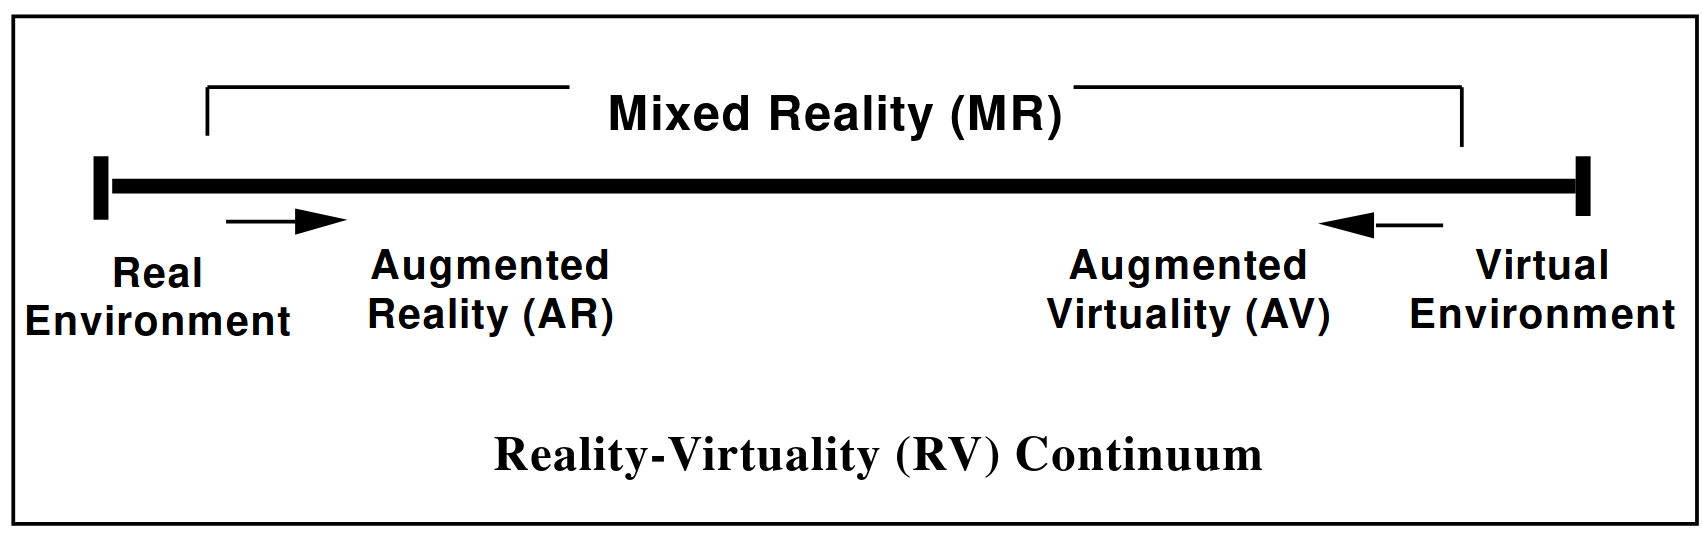
\includegraphics[width=12cm]{img/continuum.png}
  \caption{Zjednodušená reprezentácia RV kontinua \cite{milgramAugmentedRealityClass1995}.}
  \label{rv-continuum}
\end{figure}	


\subsubsection{Synonym}
V mnohých článkoch, ktoré autori \cite{speicherWhatMixedReality2019a} skúmali, sa používalo \acrshort{mr} ako synonymum pre \acrshort{ar}. To znamená, že tieto pojmy sa 
navzájom zamieňali; \acrshort{mr} bolo použité na označenie systému, ktorý jednoznačne spadal pod \acrshort{ar}, alebo bola použitá definícia \acrshort{ar} na popísanie toho,
čo niektorí autori skúmaných článkov chápali pod pojmom \acrshort{mr}.

\subsubsection{Collaboration}
\subsubsection{Combination}


\subsubsection{Alignment}

\subsubsection{Strong \acrshort{ar}}
Posledný pohľad na túto problematiku chápe \acrshort{mr} ako \emph{silnejšiu} verziu \acrshort{ar}. Zmiešaná realita je tu charakterizovaná pokročilým vnímaním prostredia
a pokročilými interakciami medzi používateľom a virtuálnymi objektmi, ako aj medzi virtuálnymi objektmi a prostredím. To vytvára predpoklad, že \acrshort{mr} závisí
na konkrétnom hardvéri alebo zariadení, ktoré dokáže poskytnúť požadovanú funkcionalitu. Taktiež sa predpokladá, že \emph{obyčajné} \acrshort{ar} nemá takéto schopnosti,
a tým pádom je \acrshort{mr} evolúciou \acrshort{ar}.



%Pomerne známym zástupcom prvého z~uvedených prístupov k rozšírenej realite je zariadenie od spoločnosti Google s~názvom Google Glass. Zariadenie v~tvare bežných 
%okuliarov, dostupné len počas pomerne krátkeho obdobia (2013 - 2015) \cite{brigham_reality_2017} dokázalo používateľovi zobrazovat informácie na malom displeji tesne
%nad pravým okom. 